% DietSense -- IEEE conference paper draft v2 (REVISED)
% Content source: openspec/changes/add-dietsense-agent (specs + design.md) and docs/01-07.
% Every finding in paper/review/review-report.md was addressed in this version.
\documentclass[conference]{IEEEtran}
\IEEEoverridecommandlockouts
\usepackage{iftex}
\ifXeTeX
  % Local build with Tectonic (XeTeX): use Times-like fonts.
  \usepackage{fontspec}
  \setmainfont{texgyretermes}[Extension=.otf, UprightFont=*-regular,
    BoldFont=*-bold, ItalicFont=*-italic, BoldItalicFont=*-bolditalic]
  \setmonofont{texgyrecursor}[Extension=.otf, UprightFont=*-regular,
    BoldFont=*-bold, ItalicFont=*-italic, BoldItalicFont=*-bolditalic]
\else
  % Overleaf (pdfLaTeX): IEEEtran already uses Times.
  \usepackage[T1]{fontenc}
\fi
\usepackage{cite}
\usepackage{amsmath,amssymb}
\usepackage{graphicx}
\usepackage{booktabs}
\usepackage{array}
\usepackage{tabularx}
\usepackage{xcolor}
\usepackage{algorithm}
\usepackage[noend]{algpseudocode}
\usepackage{tikz}
\usetikzlibrary{positioning,arrows.meta,fit,calc}
\usepackage[hidelinks]{hyperref}

\newcommand{\cn}[1]{\tikz[baseline=(c.base)]\node[circle,draw,inner sep=0.5pt,font=\scriptsize](c){#1};}
\algrenewcommand\algorithmiccomment[1]{\hfill{\footnotesize$\triangleright$ #1}}

\begin{document}

\title{DietSense: A Data-Grounded Conversational AI Agent With Uncertainty Intervals and Safety Guards for Calorie Intake Logging in Taiwan}

\author{\IEEEauthorblockN{Yen-Kai Chen}
\IEEEauthorblockA{Department of Electrical Engineering\\National Chung Hsing University\\
Taichung, Taiwan}}

\maketitle

\begin{abstract}
Dietary self-monitoring is associated with weight loss, yet adherence declines quickly: among MyFitnessPal users, logging frequency falls from 5.4 to 1.4 days per week within 12 weeks. Photo-based apps and large language models (LLMs) reduce the logging burden but remain unreliable for mixed dishes, with a mean absolute percentage error of about 36\% for GPT-4o on meal photographs and underestimation of up to 76\% for bubble milk tea, and their values are untraceable. This paper proposes DietSense, a conversational domain AI agent for calorie intake logging in Taiwan. An LLM planner performs only intent classification, food extraction, and tool orchestration. All nutrient values are retrieved from the Taiwan Food and Drug Administration food composition database, a curated Taiwanese dish database, and USDA FoodData Central, and are computed deterministically with portion conversion tables and the Mifflin--St Jeor equation. Each estimate is a low--point--high interval that widens as retrieval confidence decreases or portion descriptions become vaguer, and the agent asks at most one clarification question per food item. A rule-based safety guard evaluates intake over completed days or seven-day averages against sex-specific minimums and declines very-low-calorie plan requests. The evaluation plan comprises a 500-item annotated benchmark of Taiwanese dishes, comparisons with direct LLM estimation and manual database lookup, interval coverage analysis, a seven-day crossover user study with 20 participants, and a safety test suite. Expected outcomes, to be verified experimentally, include higher $\pm$20\% accuracy than direct LLM estimation, shorter logging time than manual lookup, and a System Usability Scale score above 70.
\end{abstract}

\begin{IEEEkeywords}
Calorie estimation, conversational agents, dietary assessment, large language models, retrieval-augmented generation, uncertainty quantification
\end{IEEEkeywords}

\section{Introduction}

Obesity is now a global chronic-disease problem: in 2024, 2.6 billion adults (45\%) were overweight, including 940 million living with obesity, and worldwide obesity prevalence more than doubled between 1990 and 2024~\cite{who_fact}. In Taiwan, the 2017--2020 Nutrition and Health Survey reported combined overweight and obesity of 58.4\% in men and 42.6\% in women~\cite{hpa_prev}, and 68.0\% of adults eat out at least seven times a week~\cite{nahsit_report}. Eating out is exactly where portion sizes and cooking oil are hardest to judge.

Dietary self-monitoring is a cornerstone of behavioral weight management; a systematic review found a consistent association between self-monitoring and weight loss~\cite{burke2011}. The difficulty is keeping it up. A scoping review of calorie-counting apps reports that MyFitnessPal logging dropped from about 5.4 to 1.4 days per week between weeks 4 and 12~\cite{dugas2026}, and users who do log omit about 18\% of food items~\cite{chen2019}. Newer tools lower the burden but not the error. GPT-4o estimates energy from standardized meal photographs with a mean absolute percentage error (MAPE) of 35.8\%~\cite{fridolfsson2025}; the best model on a Chinese-cuisine benchmark still has a MAPE of 24.45\%~\cite{jin2026}; AI image recognition underestimated bubble milk tea by up to 76\%~\cite{li2024}; and preliminary results from a metabolic-kitchen study show four popular photo apps underestimating energy by about 250--345~kcal and fat by about 30\,g per meal~\cite{hengist2026}. Numbers produced directly by an LLM also have no traceable source, and in a case study of four hypothetical adolescents with overweight or obesity, meal plans from five AI chatbots provided about 695~kcal per day less than dietitian plans~\cite{bilen2026}.

We therefore ask: \emph{how can Taiwanese users log what they eat with minimal effort while receiving calorie estimates that are sourced, honest about uncertainty, and safe?} Four obstacles stand in the way: searching large food databases, vague household portions (``a bowl''), mixed dishes, and poor coverage of Taiwanese street food in common databases~\cite{tfda_db,usda_fdc}.

This paper makes four contributions:
\begin{itemize}
\item \textbf{System design.} DietSense, a conversational domain AI agent in which the LLM only interprets language and plans tool calls, while every nutrient value comes from a database and deterministic code (Section~\ref{sec:system}).
\item \textbf{Uncertainty model.} A confidence- and vagueness-dependent interval for each item and an aggregation rule for daily totals, evaluated by both coverage and width.
\item \textbf{Safety guard.} Rules that judge low intake only on completed days or seven-day averages with sex-specific minimums, avoiding the mid-day false alarms of a naive running-total check.
\item \textbf{Evaluation protocol.} A 500-item Taiwanese dish benchmark with three-layer reference verification, two baselines, paired statistics, a user study, and a safety test suite (Section~\ref{sec:eval}).
\end{itemize}
The design is specified as testable requirements with OpenSpec; all outcomes reported here are expected, not measured.

\section{Related Work}

\subsection{AI Technology}

\textbf{Text-based estimation.} NutriBench evaluates 12 LLMs on 11{,}857 meal descriptions derived from real dietary-intake data~\cite{hua2025}. GPT-4o with chain-of-thought (CoT) prompting reached 66.8\% accuracy (carbohydrate error within $\pm$7.5\,g), comparable to or better than three nutritionists and much faster. Three findings matter here: GPT models were more accurate with metric portions (``80\,g of rice'') than with natural portions (``a cup of rice''); retrieval-augmented generation (RAG) did not always help; and error varied widely across countries.

\textbf{Image-based estimation.} ChatGPT-4 identified foods in photographs with about 93\% precision, but its nutrient estimates agreed only moderately with dietitians (intraclass correlation coefficient, ICC, 0.31--0.67)~\cite{ohara2025}. On 52 standardized photographs, GPT-4o and Claude~3.5 Sonnet both had an energy MAPE of 35.8\% and Gemini~1.5 Pro 64.2\%~\cite{fridolfsson2025}. A Taiwanese team showed that a customized Diabot-GPT-4o raised image-only food identification from 59\% to 74\%~\cite{chen2025}, and on DiningBench, a 3{,}021-dish benchmark of which 2{,}086 dishes are Chinese, the best model still has a nutrition MAPE of 24.45\%~\cite{jin2026}. GPT-4V can use language prompts to recognize regional dishes and surrounding objects to infer portion size~\cite{lo2024}, and adding contextual metadata (location, time, food items) reduces estimation error~\cite{coburn2025}.

\textbf{Data-grounded agents.} ChatDiet combines an LLM with personal and population models through an orchestrator~\cite{yang2024}. A Slovenian study evaluated four LLMs at turning natural-language questions into metadata filters over a national food composition database; easy and moderate queries were handled well but difficult ones were not~\cite{pozarnik2026}. Open-KNEAD decomposes meals and grounds each item in USDA food codes, and notably finds that recent multimodal LLMs can match full retrieval pipelines~\cite{coburn2026}. This counter-evidence is why we treat direct LLM estimation as a mandatory baseline rather than assuming retrieval wins.

\subsection{Domain Knowledge}

\textbf{Self-monitoring and its error.} MyFitnessPal shows strong correlation with a national composition database for energy ($r=0.96$) after cleaning~\cite{evenepoel2020}, yet free-living users omit items and underestimate energy~\cite{chen2019}. In food records and 24-h recalls, about 30\% of participants are under-reporters and energy is underestimated by about 15\%~\cite{poslusna2009}. Reducing the burden of each entry may therefore improve data quality more than perfecting a single estimate.

\textbf{Energy balance and requirements.} Body weight responds dynamically to energy imbalance, so a fixed ``7{,}700\,kcal per kilogram'' rule is inappropriate~\cite{hall2011}; an isocaloric ketogenic diet did not accelerate fat loss in a metabolic ward~\cite{hall2016}, and healthy low-fat and low-carbohydrate diets produced similar 12-month weight loss~\cite{gardner2018}. We use the Mifflin--St Jeor equation, developed in healthy adults, for resting energy~\cite{mifflin1990}. Individual glycemic responses differ widely~\cite{zeevi2015}, but such personalization needs glucose monitoring and is out of scope.

\textbf{Guidelines and composition data.} Taiwan's Daily Food Guide targets 50--60\% of energy from carbohydrate, 10--20\% from protein and 20--30\% from fat~\cite{hpa_guide}. The food composition database of the Taiwan Food and Drug Administration (TFDA) covers mainly raw and minimally processed foods~\cite{tfda_db}; FoodData Central of the U.S. Department of Agriculture (USDA) is broad but lacks Taiwanese street food~\cite{usda_fdc}.

\begin{table*}[t]
\caption{Article Summary of Representative Studies}
\label{tab:summary}
\centering
\footnotesize
\setlength{\tabcolsep}{3pt}
\begin{tabularx}{\textwidth}{@{}l c *{5}{>{\raggedright\arraybackslash}X}@{}}
\toprule
Ref. & Year & Problem & AI method & Data & Findings & Limitation \\
\midrule
Hua~\cite{hua2025} & 2025 & Carbohydrate from meal text & 12 LLMs; CoT, RAG & NutriBench, 11{,}857 descriptions & GPT-4o + CoT 66.8\% within $\pm$7.5\,g & Carbohydrate only; not Taiwanese food \\
O'Hara~\cite{ohara2025} & 2025 & Nutrients from photos vs.\ dietitians & ChatGPT-4 & 114 meal photos & 93\% food precision; ICC 0.31--0.67 & Small sample; moderate agreement \\
Fridolfsson~\cite{fridolfsson2025} & 2025 & Weight and energy from photos & GPT-4o, Claude 3.5, Gemini 1.5 & 52 standardized photos & Energy MAPE 35.8--64.2\% & Standardized photos; no grounding \\
Chen~\cite{chen2025} & 2025 & Customized LLM in Taiwan & Diabot-GPT-4o & 57 trainees, 714 photos & Identification 74\% vs.\ 59\% & Dietetic trainees; photos needed \\
Jin~\cite{jin2026} & 2026 & Dietary perception and reasoning & Multimodal LLMs & 3{,}021 dishes (2{,}086 Chinese) & Best nutrition MAPE 24.45\% & Image only \\
Coburn~\cite{coburn2026} & 2026 & Database-grounded estimation & Agentic decomposition + USDA FNDDS codes & Meal-image benchmark & Recent multimodal LLMs match retrieval & U.S. codes; preprint \\
Dugas~\cite{dugas2026} & 2026 & Use of calorie-counting apps & (scoping review) & Studies 2013--2024 & MyFitnessPal logging 5.4$\rightarrow$1.4 days/week & No pooled effect size \\
Chen~\cite{chen2019} & 2019 & App logging accuracy & (none) & 4-day app records vs.\ 24-h recalls & 18\% items omitted; energy underestimated & Australian adults \\
Poslusna~\cite{poslusna2009} & 2009 & Misreporting in food records & (review) & 37 studies & $\sim$30\% under-reporters; energy $-$15\% & Paper-based methods \\
\bottomrule
\end{tabularx}
\end{table*}

\subsection{Research Gap}
Table~\ref{tab:summary} shows four gaps: (G1) estimators that are both low-burden and traceable; (G2) grounding data for Taiwanese cooked dishes; (G3) calibrated uncertainty rather than single point estimates; and (G4) conversational logging that is both low-burden and safe. DietSense addresses each in turn with source-anchored values, a Taiwan-first retrieval order, calibrated intervals, and a bounded clarification loop with a safety guard.

\section{Proposed System}
\label{sec:system}

\subsection{Architecture}

\begin{figure*}[t]
\centering
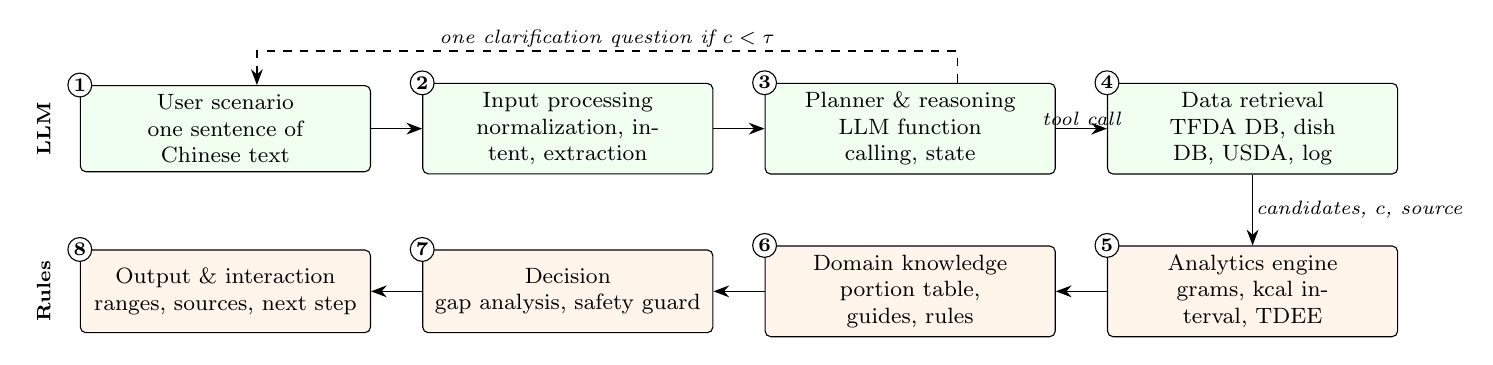
\begin{tikzpicture}[
  box/.style={draw, rounded corners=2pt, align=center, font=\footnotesize, minimum height=1.05cm, text width=3.45cm, fill=#1},
  box/.default={green!6},
  num/.style={circle, draw, fill=white, inner sep=0.8pt, font=\scriptsize\bfseries},
  arr/.style={-{Stealth[length=2mm]}, semithick},
  lab/.style={font=\scriptsize\itshape, inner sep=1pt}]
\node[box] (m1) {User scenario\\ one sentence of Chinese text};
\node[box, right=0.65cm of m1] (m2) {Input processing\\ normalization, intent, extraction};
\node[box, right=0.65cm of m2] (m3) {Planner \& reasoning\\ LLM function calling, state};
\node[box, right=0.65cm of m3] (m4) {Data retrieval\\ TFDA DB, dish DB, USDA, log};
\node[box=orange!8, below=0.9cm of m4] (m5) {Analytics engine\\ grams, kcal interval, TDEE};
\node[box=orange!8, left=0.65cm of m5] (m6) {Domain knowledge\\ portion table, guides, rules};
\node[box=orange!8, left=0.65cm of m6] (m7) {Decision\\ gap analysis, safety guard};
\node[box=orange!8, left=0.65cm of m7] (m8) {Output \& interaction\\ ranges, sources, next step};
\foreach \i in {1,...,8} \node[num] at (m\i.north west) {\i};
\draw[arr] (m1) -- (m2); \draw[arr] (m2) -- (m3); \draw[arr] (m3) -- node[lab, above]{tool call} (m4);
\draw[arr] (m4) -- node[lab, right]{candidates, $c$, source} (m5);
\draw[arr] (m5) -- (m6); \draw[arr] (m6) -- (m7); \draw[arr] (m7) -- (m8);
\draw[arr, dashed] ($(m3.north)+(0.6,0)$) -- ++(0,0.4) -| node[lab, above, pos=0.25]{one clarification question if $c<\tau$} ($(m1.north)+(0.4,0)$);
\node[font=\scriptsize\bfseries, rotate=90, anchor=south] at ($(m1.west)+(-0.25,0)$) {LLM};
\node[font=\scriptsize\bfseries, rotate=90, anchor=south] at ($(m8.west)+(-0.25,0)$) {Rules};
\end{tikzpicture}
\caption{DietSense architecture. Top row: language understanding and retrieval; the LLM never produces nutrient values. Bottom row: deterministic computation and decisions.}
\label{fig:arch}
\end{figure*}

Fig.~\ref{fig:arch} shows the eight modules. \cn{1}~Users are Taiwanese adults who mostly eat out and describe a meal in one sentence; a profile (sex, age, height, weight, activity) is collected once. \cn{2}~Deterministic normalization (script, full/half width, ``half a bowl''$\rightarrow$0.5 bowl) is followed by one structured LLM call that returns an intent (\texttt{log\_food}, \texttt{query\_nutrition}, \texttt{analyze}, \texttt{recommend}) and entities (food, portion, modifiers, meal); invalid JSON is retried once. \cn{3}~The planner decides which tools to call, keeps the dialogue state (including a per-item \texttt{asked} flag), and either calls a tool, asks one question, or responds; it produces no numbers. \cn{4}~Retrieval queries, in order, Taiwan's food composition dataset~\cite{tfda_db}, a curated dish database whose entries list ingredients, grams and the matching official item, and USDA FoodData Central~\cite{usda_fdc}; a source that times out is skipped and the response says so. \cn{5}~The analytics engine converts portions to grams, sums energy per ingredient, computes intervals, macronutrient shares, basal metabolic rate (BMR) and total daily energy expenditure (TDEE); missing profile fields are requested from the user, never filled with defaults. \cn{6}~Domain knowledge is stored as tables and rules, not prompts: portion tables by food category, the Daily Food Guide ranges~\cite{hpa_guide}, the Mifflin--St Jeor equation~\cite{mifflin1990}, and safety minimums~\cite{harvard2024}. \cn{7}~Decisions run the safety guard first and only then compute gap analysis and substitutions. \cn{8}~Each response shows item intervals, the daily total versus TDEE, expandable sources (database and item ID), and the next step.

\subsection{Retrieval Confidence and Fallback}
Each candidate receives a confidence $c\in[0,1]$ combining name similarity (exact alias match or embedding similarity) and attribute consistency (category, cooking method, unit). If $c<\tau=0.80$ and the item has not yet been questioned, the agent asks one clarification question and retrieves again. If $c$ remains below $\tau_{\text{low}}=0.50$, the LLM may propose ingredients and proportions, but per-100\,g values are still looked up in the database, and the entry is labeled \emph{approximate}. Both thresholds are initial values to be calibrated in the evaluation.

\subsection{Calorie Intervals}
For item $m$ with portion $g$ grams, ingredient weight shares $s_j$, energy densities $\rho_j$ (kcal/100\,g) and modifier adjustments $a_j$ (e.g., $a=0.5$ for ``half of the soup''),
\begin{equation}
k=\sum_j g\, s_j\, \rho_j\, a_j/100 .
\end{equation}
The relative half-width grows with low confidence and vague portions,
\begin{equation}
w=\min\!\bigl(w_{\max},\; w_0+\alpha(1-c)+\beta v\bigr),
\end{equation}
where $v=0$ for grams or labeled packages, $0.5$ for household units and $1$ when no portion is given; $w_0=0.10$, $\alpha=0.50$, $\beta=0.15$ and $w_{\max}=0.60$. The item interval is $[k(1-w),\,k,\,k(1+w)]$. For a day with items $i$, point estimates add and absolute half-widths combine as
\begin{equation}
\label{eq:day}
K=\sum_i k_i,\qquad \Delta=\sqrt{\textstyle\sum_i (k_i w_i)^2},
\end{equation}
giving the daily interval $[K-\Delta,\,K,\,K+\Delta]$. Simple addition of bounds would assume every item errs in the same direction and make the interval grow with the number of entries. Because self-report errors may in fact be correlated~\cite{poslusna2009}, day-level coverage is evaluated separately. Energy requirement uses $\text{BMR}=10\,\text{weight}+6.25\,\text{height}-5\,\text{age}+5$ for men and $-161$ instead of $+5$ for women (kg, cm, years)~\cite{mifflin1990}; TDEE is BMR multiplied by an activity factor of 1.2--1.9.

\subsection{Safety Guard}
Low intake is judged only after the day is closed (user confirmation or 04:00 the next day) or on a seven-day average, so a 350\,kcal breakfast never triggers an alert. Minimums are 1{,}200\,kcal for women and 1{,}500\,kcal for men~\cite{harvard2024}; if sex is unknown the agent asks and applies 1{,}200\,kcal until answered. Requests for plans below the minimum are declined with an explanation. Two or more occurrences within seven days of a day above 150\% of TDEE followed by a day below 50\% trigger a nonjudgmental prompt with support resources. When any rule fires, the agent gives no further restriction advice. A non-medical disclaimer is shown at first use and with every alert.

\subsection{Algorithm}
Algorithm~\ref{alg:agent} gives the complete control flow. Its safeguards are a query-only branch that never writes to the log (line~4), clarification bounded to one question per item (lines~9--10), a fallback for unresolved items (line~11), a daily state computed once and shared by every branch (line~16), and a safety check that uses only completed-day or seven-day data (line~17).

\begin{algorithm}[t]
\caption{DietSense agent}
\label{alg:agent}
\footnotesize
\begin{algorithmic}[1]
\Require message $Q$, profile $P$, daily log $D$, 7-day history $H$
\Ensure response $R$, updated log $D$
\State $q\gets$ \Call{Normalize}{$Q$}
\State $(\mathit{intent},E)\gets$ \Call{ClassifyExtract}{$q$} \Comment{LLM}
\If{$\mathit{intent}=\textsc{unknown}$} \Return \Call{Ask}{log or query?}, $D$ \EndIf
\If{$\mathit{intent}=\texttt{query\_nutrition}$} \Return \Call{Render}{\textsc{Lookup}$(E)$}, $D$ \EndIf
\If{$\mathit{intent}=\texttt{log\_food}$}
  \For{each $e\in E$}
    \State $C\gets$ \Call{Retrieve}{$e$, [TFDA, Dish, USDA]}
    \State $(m,c)\gets$ \Call{Rank}{$C,e$}
    \If{$c<\tau$ \textbf{and not} $e.\mathit{asked}$}
      \State $e\gets$ \Call{Ask}{\textsc{Clarify}$(e,C)$}; $e.\mathit{asked}\gets$ true; \textbf{goto} 7
    \EndIf
    \If{$c<\tau_{\text{low}}$} $m\gets$ \Call{Decompose}{$e$}; $e.\mathit{approx}\gets$ true \EndIf
    \State $g\gets$ \Call{PortionToGrams}{$e,m$} \Comment{portion table}
    \State $k\gets \sum_j g\,s_j \rho_j a_j/100$
    \State $w\gets\min(w_{\max},w_0+\alpha(1-c)+\beta v(e))$
    \State $D$.add$(m,g,[k(1-w),k,k(1+w)],\mathit{source},c)$
  \EndFor
\EndIf
\State $S\gets$ \Call{DailyState}{$D,P$} \Comment{totals, macros, TDEE}
\State $r\gets$ \Call{SafetyCheck}{$D,H,P,S,q$} \Comment{closed day / 7-day}
\If{$r\neq\textsc{ok}$} \Return \Call{Render}{\textsc{Alert}$(r)$}, $D$ \EndIf
\State $\mathit{rec}\gets$ \Call{Recommend}{$S,P$} \textbf{if} $\mathit{intent}\in\{\texttt{analyze},\texttt{recommend}\}$ \textbf{else} $\varnothing$
\State \Return \Call{Render}{$S,\mathit{rec}$, sources, intervals}, $D$
\end{algorithmic}
\end{algorithm}

\subsection{Worked Example}
A 30-year-old woman (165\,cm, 60\,kg, activity 1.55) who logged a 380\,kcal breakfast types ``lunch was a bowl of Taiwanese beef noodles with an egg, half of the soup.'' The noodles match a dish entry with $c=0.86$; the egg ($c=0.72$) triggers one question (braised or fried?) and, after ``braised'', $c=0.93$. With illustrative values, the beef noodle soup sums to $340+160+0.5\times250=625$\,kcal (noodles, beef, and half of the soup; $w=0.245$) and the egg to 75\,kcal ($w=0.21$), giving a meal of 700\,kcal with range 546--854\,kcal by \eqref{eq:day}. Including the breakfast entries, the day stands at 1{,}080\,kcal (913--1{,}247) against a TDEE of about 2{,}046\,kcal; because the day is open, no low-intake alert is raised. These numbers illustrate the computation and are not measurements.

\section{Evaluation Plan}
\label{sec:eval}

\subsection{Benchmark and Reference Values}
We will build 500 natural-language descriptions of Taiwanese meals, with at least 30 items in each known high-error category (bubble tea and other mixed drinks, noodle soups, thickened rice dishes, fried food). All reference values are computed by ingredient decomposition from the official database with documented recipes. At least 50 items (10\%) are computed independently by two annotators, reporting the share within 10\% and arbitrating larger gaps; at least 30 items are checked against vendor nutrition labels, and items deviating by more than 20\% are excluded until resolved. No dietitian review is available, which we report as a limitation.

\subsection{Baselines, Metrics and Statistics}
Baselines are (i) direct LLM estimation with the same model, without database access, using both base and CoT prompts, since CoT substantially improves direct estimation~\cite{hua2025}; and (ii) manual lookup in the official database by an operator not involved in annotation, on a stratified sample of at least 100 items. Accuracy is measured by mean absolute error (MAE), MAPE and $\pm$10\%/$\pm$20\% hit rates, overall and per category. Uncertainty is measured by interval coverage and mean half-width at both item and day level; reporting both prevents buying coverage with very wide intervals. Paired comparisons use McNemar's test for hit rates and paired bootstrap 95\% confidence intervals for errors. The safety suite contains at least 30 unsafe requests and risk patterns, including male, female and unknown-sex cases, and reports block and false-alarm rates.

\subsection{User Study}
Twenty adults will use DietSense and a conventional app for seven days in a counterbalanced within-subject crossover, recording seconds per meal, clarification rate, days logged, and the System Usability Scale (SUS). Participants give written consent, data stay de-identified and local, and minors, pregnant women and people with a history of eating disorders are excluded by screening.

\subsection{Expected Outcomes}
These are targets for the proposal stage, not results: higher $\pm$20\% hit rate than the direct-LLM baseline; item-level coverage of at least 80\% with reported width; shorter logging time than manual lookup; SUS above 70; and a 100\% block rate on the safety suite.

\section{Feasibility and Limitations}
Taiwan's food composition dataset is openly licensed and updated quarterly in CSV, JSON and XML~\cite{tfda_db}; USDA FoodData Central offers a public-domain API limited to 1{,}000 requests per hour per IP, handled with local caching~\cite{usda_fdc}. The dish database ($\geq$150 dishes) and the benchmark are estimated at about 50 hours each, the main schedule risk; if needed, voice input (a stretch goal) and user-study size are reduced first, while the safety guard and source tracing are never cut. Limitations include text-only input, residual self-report bias, the absence of dietitian review, and minimums based on sex only; minimums are general adult references, and pregnant users, athletes and older adults are directed to professionals.

\section{Conclusion}
DietSense separates language understanding from nutrient computation so that every calorie value is traceable, expressed as a calibrated range, and filtered by explicit safety rules. The evaluation plan tests whether this design remains worthwhile against direct LLM estimation, an open question raised by recent work~\cite{coburn2026}. Future work includes image input, micronutrients, and minimums adjusted to body composition.

\bibliographystyle{IEEEtran}
\bibliography{references}

\end{document}
